\documentclass{article}
\usepackage{tikz}
\begin{document}
% measure how TikZ reads bare numbers for circle radii and shifts
\newsavebox{\boxa}\newsavebox{\boxb}\newsavebox{\boxc}\newsavebox{\boxd}
\savebox{\boxa}{\hbox{\begin{tikzpicture}[x=2cm,y=2cm]\draw (0,0) circle (1);\end{tikzpicture}}}
\savebox{\boxb}{\hbox{\begin{tikzpicture}[x=2cm,y=2cm]\draw (0,0) circle (2cm);\end{tikzpicture}}}
\savebox{\boxc}{\hbox{\begin{tikzpicture}\draw (0,0) -- (1,0);\end{tikzpicture}}}
\savebox{\boxd}{\hbox{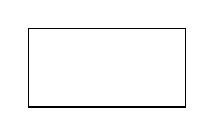
\begin{tikzpicture}[x=2cm,y=1cm]\draw (0,0) rectangle (1,1);\end{tikzpicture}}}
\typeout{MEASURE circle-bare=\the\wd\boxa\space circle-cm=\the\wd\boxb
  \space unitline=\the\wd\boxc\space rect=\the\wd\boxd\space rectHT=\the\ht\boxd}
% arc radius bare number
\newsavebox{\boxe}\newsavebox{\boxf}
\savebox{\boxe}{\hbox{\begin{tikzpicture}[x=2cm,y=2cm]\draw (0,0) arc[start angle=0,end angle=90,radius=1];\end{tikzpicture}}}
\savebox{\boxf}{\hbox{\begin{tikzpicture}[x=2cm,y=2cm]\begin{scope}[xshift=1]\draw (0,0) circle (1pt);\end{scope}\end{tikzpicture}}}
\typeout{MEASURE arc-bare=\the\wd\boxe\space scope-xshift-in-scaled=\the\wd\boxf}
\end{document}
